\documentclass[tikz, border=1mm]{standalone}
\begin{document}
\begin{minipage}{\textwidth}
\centering
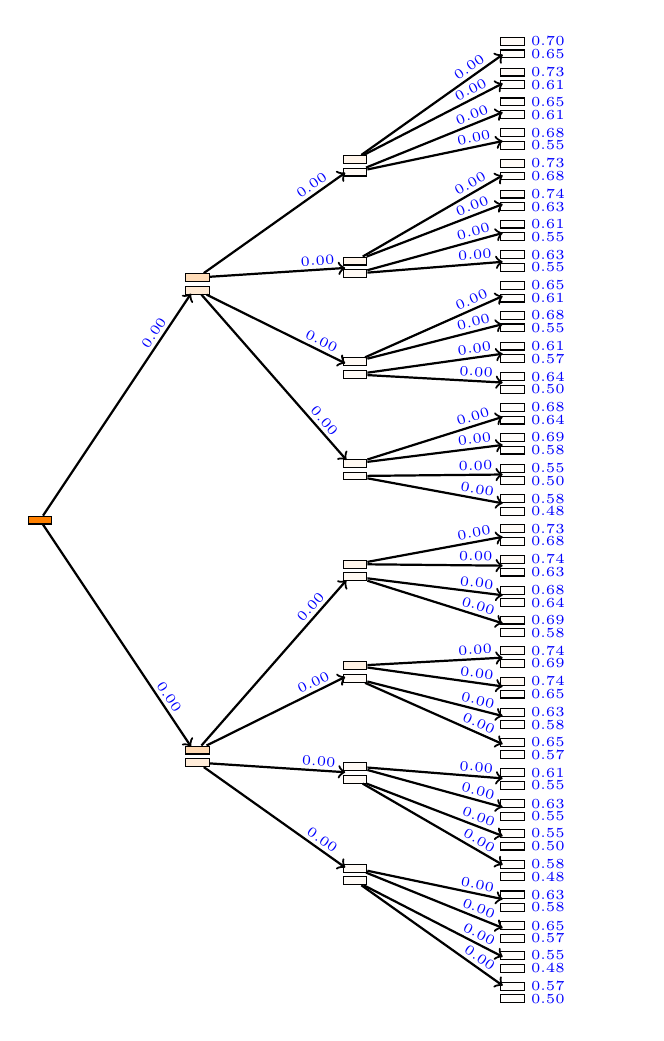
\begin{tikzpicture}
\tikzstyle{between} = [rectangle, draw=none]
\tikzstyle{qval}    = [rectangle, text centered, text width=2cm]
\node[between] at (-8.00, 3.00) (1_b_0){};
\node[between] at (-8.00, -3.00) (1_b_1){};
\node[between] at (-6.00, 4.50) (2_b_0){};
\node[between] at (-6.00, 3.21) (2_b_1){};
\node[between] at (-6.00, 1.93) (2_b_2){};
\node[between] at (-6.00, 0.64) (2_b_3){};
\node[between] at (-6.00, -0.64) (2_b_4){};
\node[between] at (-6.00, -1.93) (2_b_5){};
\node[between] at (-6.00, -3.21) (2_b_6){};
\node[between] at (-6.00, -4.50) (2_b_7){};
\node[between] at (-4.00, 6.00) (3_b_0){};
\node[between] at (-4.00, 5.61) (3_b_1){};
\node[between] at (-4.00, 5.23) (3_b_2){};
\node[between] at (-4.00, 4.84) (3_b_3){};
\node[between] at (-4.00, 4.45) (3_b_4){};
\node[between] at (-4.00, 4.06) (3_b_5){};
\node[between] at (-4.00, 3.68) (3_b_6){};
\node[between] at (-4.00, 3.29) (3_b_7){};
\node[between] at (-4.00, 2.90) (3_b_8){};
\node[between] at (-4.00, 2.52) (3_b_9){};
\node[between] at (-4.00, 2.13) (3_b_10){};
\node[between] at (-4.00, 1.74) (3_b_11){};
\node[between] at (-4.00, 1.35) (3_b_12){};
\node[between] at (-4.00, 0.97) (3_b_13){};
\node[between] at (-4.00, 0.58) (3_b_14){};
\node[between] at (-4.00, 0.19) (3_b_15){};
\node[between] at (-4.00, -0.19) (3_b_16){};
\node[between] at (-4.00, -0.58) (3_b_17){};
\node[between] at (-4.00, -0.97) (3_b_18){};
\node[between] at (-4.00, -1.35) (3_b_19){};
\node[between] at (-4.00, -1.74) (3_b_20){};
\node[between] at (-4.00, -2.13) (3_b_21){};
\node[between] at (-4.00, -2.52) (3_b_22){};
\node[between] at (-4.00, -2.90) (3_b_23){};
\node[between] at (-4.00, -3.29) (3_b_24){};
\node[between] at (-4.00, -3.68) (3_b_25){};
\node[between] at (-4.00, -4.06) (3_b_26){};
\node[between] at (-4.00, -4.45) (3_b_27){};
\node[between] at (-4.00, -4.84) (3_b_28){};
\node[between] at (-4.00, -5.23) (3_b_29){};
\node[between] at (-4.00, -5.61) (3_b_30){};
\node[between] at (-4.00, -6.00) (3_b_31){};
\node[rectangle, text centered, draw=black, minimum height=1mm, text width=3mm, inner sep=0pt, fill=orange, fill opacity=1.00, draw opacity=1] at (-10.00, 0.00) (0_s_0){};
\node[rectangle, text centered, draw=black, minimum height=1mm, text width=3mm, inner sep=0pt, fill=orange, fill opacity=0.28, draw opacity=1] at (-8.00, 3.08) (1_s_0) {};
\node[rectangle, text centered, draw=black, minimum height=1mm, text width=3mm, inner sep=0pt, fill=orange, fill opacity=0.17, draw opacity=1] at (-8.00, 2.92) (1_s_1) {};
\node[rectangle, text centered, draw=black, minimum height=1mm, text width=3mm, inner sep=0pt, fill=orange, fill opacity=0.30, draw opacity=1] at (-8.00, -2.92) (1_s_2) {};
\node[rectangle, text centered, draw=black, minimum height=1mm, text width=3mm, inner sep=0pt, fill=orange, fill opacity=0.15, draw opacity=1] at (-8.00, -3.08) (1_s_3) {};
\node[rectangle, text centered, draw=black, minimum height=1mm, text width=3mm, inner sep=0pt, fill=orange, fill opacity=0.08, draw opacity=1] at (-6.00, 4.58) (2_s_0) {};
\node[rectangle, text centered, draw=black, minimum height=1mm, text width=3mm, inner sep=0pt, fill=orange, fill opacity=0.04, draw opacity=1] at (-6.00, 4.42) (2_s_1) {};
\node[rectangle, text centered, draw=black, minimum height=1mm, text width=3mm, inner sep=0pt, fill=orange, fill opacity=0.08, draw opacity=1] at (-6.00, 3.29) (2_s_2) {};
\node[rectangle, text centered, draw=black, minimum height=1mm, text width=3mm, inner sep=0pt, fill=orange, fill opacity=0.04, draw opacity=1] at (-6.00, 3.13) (2_s_3) {};
\node[rectangle, text centered, draw=black, minimum height=1mm, text width=3mm, inner sep=0pt, fill=orange, fill opacity=0.04, draw opacity=1] at (-6.00, 2.01) (2_s_4) {};
\node[rectangle, text centered, draw=black, minimum height=1mm, text width=3mm, inner sep=0pt, fill=orange, fill opacity=0.03, draw opacity=1] at (-6.00, 1.85) (2_s_5) {};
\node[rectangle, text centered, draw=black, minimum height=1mm, text width=3mm, inner sep=0pt, fill=orange, fill opacity=0.05, draw opacity=1] at (-6.00, 0.72) (2_s_6) {};
\node[rectangle, text centered, draw=black, minimum height=1mm, text width=3mm, inner sep=0pt, fill=orange, fill opacity=0.03, draw opacity=1] at (-6.00, 0.56) (2_s_7) {};
\node[rectangle, text centered, draw=black, minimum height=1mm, text width=3mm, inner sep=0pt, fill=orange, fill opacity=0.08, draw opacity=1] at (-6.00, -0.56) (2_s_8) {};
\node[rectangle, text centered, draw=black, minimum height=1mm, text width=3mm, inner sep=0pt, fill=orange, fill opacity=0.05, draw opacity=1] at (-6.00, -0.72) (2_s_9) {};
\node[rectangle, text centered, draw=black, minimum height=1mm, text width=3mm, inner sep=0pt, fill=orange, fill opacity=0.10, draw opacity=1] at (-6.00, -1.85) (2_s_10) {};
\node[rectangle, text centered, draw=black, minimum height=1mm, text width=3mm, inner sep=0pt, fill=orange, fill opacity=0.03, draw opacity=1] at (-6.00, -2.01) (2_s_11) {};
\node[rectangle, text centered, draw=black, minimum height=1mm, text width=3mm, inner sep=0pt, fill=orange, fill opacity=0.04, draw opacity=1] at (-6.00, -3.13) (2_s_12) {};
\node[rectangle, text centered, draw=black, minimum height=1mm, text width=3mm, inner sep=0pt, fill=orange, fill opacity=0.03, draw opacity=1] at (-6.00, -3.29) (2_s_13) {};
\node[rectangle, text centered, draw=black, minimum height=1mm, text width=3mm, inner sep=0pt, fill=orange, fill opacity=0.03, draw opacity=1] at (-6.00, -4.42) (2_s_14) {};
\node[rectangle, text centered, draw=black, minimum height=1mm, text width=3mm, inner sep=0pt, fill=orange, fill opacity=0.03, draw opacity=1] at (-6.00, -4.58) (2_s_15) {};
\node[rectangle, text centered, draw=black, minimum height=1mm, text width=3mm, inner sep=0pt, fill=orange, fill opacity=0.03, draw opacity=1] at (-4.00, 6.08) (3_s_0) {};
\node[qval] at (-3.55, 6.08) () {\tiny \textcolor{blue}{0.70}};
\node[rectangle, text centered, draw=black, minimum height=1mm, text width=3mm, inner sep=0pt, fill=orange, fill opacity=0.01, draw opacity=1] at (-4.00, 5.92) (3_s_1) {};
\node[qval] at (-3.55, 5.92) () {\tiny \textcolor{blue}{0.65}};
\node[rectangle, text centered, draw=black, minimum height=1mm, text width=3mm, inner sep=0pt, fill=orange, fill opacity=0.03, draw opacity=1] at (-4.00, 5.69) (3_s_2) {};
\node[qval] at (-3.55, 5.69) () {\tiny \textcolor{blue}{0.73}};
\node[rectangle, text centered, draw=black, minimum height=1mm, text width=3mm, inner sep=0pt, fill=orange, fill opacity=0.01, draw opacity=1] at (-4.00, 5.53) (3_s_3) {};
\node[qval] at (-3.55, 5.53) () {\tiny \textcolor{blue}{0.61}};
\node[rectangle, text centered, draw=black, minimum height=1mm, text width=3mm, inner sep=0pt, fill=orange, fill opacity=0.01, draw opacity=1] at (-4.00, 5.31) (3_s_4) {};
\node[qval] at (-3.55, 5.31) () {\tiny \textcolor{blue}{0.65}};
\node[rectangle, text centered, draw=black, minimum height=1mm, text width=3mm, inner sep=0pt, fill=orange, fill opacity=0.01, draw opacity=1] at (-4.00, 5.15) (3_s_5) {};
\node[qval] at (-3.55, 5.15) () {\tiny \textcolor{blue}{0.61}};
\node[rectangle, text centered, draw=black, minimum height=1mm, text width=3mm, inner sep=0pt, fill=orange, fill opacity=0.01, draw opacity=1] at (-4.00, 4.92) (3_s_6) {};
\node[qval] at (-3.55, 4.92) () {\tiny \textcolor{blue}{0.68}};
\node[rectangle, text centered, draw=black, minimum height=1mm, text width=3mm, inner sep=0pt, fill=orange, fill opacity=0.01, draw opacity=1] at (-4.00, 4.76) (3_s_7) {};
\node[qval] at (-3.55, 4.76) () {\tiny \textcolor{blue}{0.55}};
\node[rectangle, text centered, draw=black, minimum height=1mm, text width=3mm, inner sep=0pt, fill=orange, fill opacity=0.03, draw opacity=1] at (-4.00, 4.53) (3_s_8) {};
\node[qval] at (-3.55, 4.53) () {\tiny \textcolor{blue}{0.73}};
\node[rectangle, text centered, draw=black, minimum height=1mm, text width=3mm, inner sep=0pt, fill=orange, fill opacity=0.01, draw opacity=1] at (-4.00, 4.37) (3_s_9) {};
\node[qval] at (-3.55, 4.37) () {\tiny \textcolor{blue}{0.68}};
\node[rectangle, text centered, draw=black, minimum height=1mm, text width=3mm, inner sep=0pt, fill=orange, fill opacity=0.03, draw opacity=1] at (-4.00, 4.14) (3_s_10) {};
\node[qval] at (-3.55, 4.14) () {\tiny \textcolor{blue}{0.74}};
\node[rectangle, text centered, draw=black, minimum height=1mm, text width=3mm, inner sep=0pt, fill=orange, fill opacity=0.01, draw opacity=1] at (-4.00, 3.98) (3_s_11) {};
\node[qval] at (-3.55, 3.98) () {\tiny \textcolor{blue}{0.63}};
\node[rectangle, text centered, draw=black, minimum height=1mm, text width=3mm, inner sep=0pt, fill=orange, fill opacity=0.01, draw opacity=1] at (-4.00, 3.76) (3_s_12) {};
\node[qval] at (-3.55, 3.76) () {\tiny \textcolor{blue}{0.61}};
\node[rectangle, text centered, draw=black, minimum height=1mm, text width=3mm, inner sep=0pt, fill=orange, fill opacity=0.01, draw opacity=1] at (-4.00, 3.60) (3_s_13) {};
\node[qval] at (-3.55, 3.60) () {\tiny \textcolor{blue}{0.55}};
\node[rectangle, text centered, draw=black, minimum height=1mm, text width=3mm, inner sep=0pt, fill=orange, fill opacity=0.01, draw opacity=1] at (-4.00, 3.37) (3_s_14) {};
\node[qval] at (-3.55, 3.37) () {\tiny \textcolor{blue}{0.63}};
\node[rectangle, text centered, draw=black, minimum height=1mm, text width=3mm, inner sep=0pt, fill=orange, fill opacity=0.01, draw opacity=1] at (-4.00, 3.21) (3_s_15) {};
\node[qval] at (-3.55, 3.21) () {\tiny \textcolor{blue}{0.55}};
\node[rectangle, text centered, draw=black, minimum height=1mm, text width=3mm, inner sep=0pt, fill=orange, fill opacity=0.01, draw opacity=1] at (-4.00, 2.98) (3_s_16) {};
\node[qval] at (-3.55, 2.98) () {\tiny \textcolor{blue}{0.65}};
\node[rectangle, text centered, draw=black, minimum height=1mm, text width=3mm, inner sep=0pt, fill=orange, fill opacity=0.01, draw opacity=1] at (-4.00, 2.82) (3_s_17) {};
\node[qval] at (-3.55, 2.82) () {\tiny \textcolor{blue}{0.61}};
\node[rectangle, text centered, draw=black, minimum height=1mm, text width=3mm, inner sep=0pt, fill=orange, fill opacity=0.01, draw opacity=1] at (-4.00, 2.60) (3_s_18) {};
\node[qval] at (-3.55, 2.60) () {\tiny \textcolor{blue}{0.68}};
\node[rectangle, text centered, draw=black, minimum height=1mm, text width=3mm, inner sep=0pt, fill=orange, fill opacity=0.01, draw opacity=1] at (-4.00, 2.44) (3_s_19) {};
\node[qval] at (-3.55, 2.44) () {\tiny \textcolor{blue}{0.55}};
\node[rectangle, text centered, draw=black, minimum height=1mm, text width=3mm, inner sep=0pt, fill=orange, fill opacity=0.01, draw opacity=1] at (-4.00, 2.21) (3_s_20) {};
\node[qval] at (-3.55, 2.21) () {\tiny \textcolor{blue}{0.61}};
\node[rectangle, text centered, draw=black, minimum height=1mm, text width=3mm, inner sep=0pt, fill=orange, fill opacity=0.01, draw opacity=1] at (-4.00, 2.05) (3_s_21) {};
\node[qval] at (-3.55, 2.05) () {\tiny \textcolor{blue}{0.57}};
\node[rectangle, text centered, draw=black, minimum height=1mm, text width=3mm, inner sep=0pt, fill=orange, fill opacity=0.01, draw opacity=1] at (-4.00, 1.82) (3_s_22) {};
\node[qval] at (-3.55, 1.82) () {\tiny \textcolor{blue}{0.64}};
\node[rectangle, text centered, draw=black, minimum height=1mm, text width=3mm, inner sep=0pt, fill=orange, fill opacity=0.01, draw opacity=1] at (-4.00, 1.66) (3_s_23) {};
\node[qval] at (-3.55, 1.66) () {\tiny \textcolor{blue}{0.50}};
\node[rectangle, text centered, draw=black, minimum height=1mm, text width=3mm, inner sep=0pt, fill=orange, fill opacity=0.01, draw opacity=1] at (-4.00, 1.43) (3_s_24) {};
\node[qval] at (-3.55, 1.43) () {\tiny \textcolor{blue}{0.68}};
\node[rectangle, text centered, draw=black, minimum height=1mm, text width=3mm, inner sep=0pt, fill=orange, fill opacity=0.01, draw opacity=1] at (-4.00, 1.27) (3_s_25) {};
\node[qval] at (-3.55, 1.27) () {\tiny \textcolor{blue}{0.64}};
\node[rectangle, text centered, draw=black, minimum height=1mm, text width=3mm, inner sep=0pt, fill=orange, fill opacity=0.02, draw opacity=1] at (-4.00, 1.05) (3_s_26) {};
\node[qval] at (-3.55, 1.05) () {\tiny \textcolor{blue}{0.69}};
\node[rectangle, text centered, draw=black, minimum height=1mm, text width=3mm, inner sep=0pt, fill=orange, fill opacity=0.01, draw opacity=1] at (-4.00, 0.89) (3_s_27) {};
\node[qval] at (-3.55, 0.89) () {\tiny \textcolor{blue}{0.58}};
\node[rectangle, text centered, draw=black, minimum height=1mm, text width=3mm, inner sep=0pt, fill=orange, fill opacity=0.01, draw opacity=1] at (-4.00, 0.66) (3_s_28) {};
\node[qval] at (-3.55, 0.66) () {\tiny \textcolor{blue}{0.55}};
\node[rectangle, text centered, draw=black, minimum height=1mm, text width=3mm, inner sep=0pt, fill=orange, fill opacity=0.01, draw opacity=1] at (-4.00, 0.50) (3_s_29) {};
\node[qval] at (-3.55, 0.50) () {\tiny \textcolor{blue}{0.50}};
\node[rectangle, text centered, draw=black, minimum height=1mm, text width=3mm, inner sep=0pt, fill=orange, fill opacity=0.01, draw opacity=1] at (-4.00, 0.27) (3_s_30) {};
\node[qval] at (-3.55, 0.27) () {\tiny \textcolor{blue}{0.58}};
\node[rectangle, text centered, draw=black, minimum height=1mm, text width=3mm, inner sep=0pt, fill=orange, fill opacity=0.01, draw opacity=1] at (-4.00, 0.11) (3_s_31) {};
\node[qval] at (-3.55, 0.11) () {\tiny \textcolor{blue}{0.48}};
\node[rectangle, text centered, draw=black, minimum height=1mm, text width=3mm, inner sep=0pt, fill=orange, fill opacity=0.03, draw opacity=1] at (-4.00, -0.11) (3_s_32) {};
\node[qval] at (-3.55, -0.11) () {\tiny \textcolor{blue}{0.73}};
\node[rectangle, text centered, draw=black, minimum height=1mm, text width=3mm, inner sep=0pt, fill=orange, fill opacity=0.01, draw opacity=1] at (-4.00, -0.27) (3_s_33) {};
\node[qval] at (-3.55, -0.27) () {\tiny \textcolor{blue}{0.68}};
\node[rectangle, text centered, draw=black, minimum height=1mm, text width=3mm, inner sep=0pt, fill=orange, fill opacity=0.03, draw opacity=1] at (-4.00, -0.50) (3_s_34) {};
\node[qval] at (-3.55, -0.50) () {\tiny \textcolor{blue}{0.74}};
\node[rectangle, text centered, draw=black, minimum height=1mm, text width=3mm, inner sep=0pt, fill=orange, fill opacity=0.01, draw opacity=1] at (-4.00, -0.66) (3_s_35) {};
\node[qval] at (-3.55, -0.66) () {\tiny \textcolor{blue}{0.63}};
\node[rectangle, text centered, draw=black, minimum height=1mm, text width=3mm, inner sep=0pt, fill=orange, fill opacity=0.01, draw opacity=1] at (-4.00, -0.89) (3_s_36) {};
\node[qval] at (-3.55, -0.89) () {\tiny \textcolor{blue}{0.68}};
\node[rectangle, text centered, draw=black, minimum height=1mm, text width=3mm, inner sep=0pt, fill=orange, fill opacity=0.01, draw opacity=1] at (-4.00, -1.05) (3_s_37) {};
\node[qval] at (-3.55, -1.05) () {\tiny \textcolor{blue}{0.64}};
\node[rectangle, text centered, draw=black, minimum height=1mm, text width=3mm, inner sep=0pt, fill=orange, fill opacity=0.02, draw opacity=1] at (-4.00, -1.27) (3_s_38) {};
\node[qval] at (-3.55, -1.27) () {\tiny \textcolor{blue}{0.69}};
\node[rectangle, text centered, draw=black, minimum height=1mm, text width=3mm, inner sep=0pt, fill=orange, fill opacity=0.01, draw opacity=1] at (-4.00, -1.43) (3_s_39) {};
\node[qval] at (-3.55, -1.43) () {\tiny \textcolor{blue}{0.58}};
\node[rectangle, text centered, draw=black, minimum height=1mm, text width=3mm, inner sep=0pt, fill=orange, fill opacity=0.03, draw opacity=1] at (-4.00, -1.66) (3_s_40) {};
\node[qval] at (-3.55, -1.66) () {\tiny \textcolor{blue}{0.74}};
\node[rectangle, text centered, draw=black, minimum height=1mm, text width=3mm, inner sep=0pt, fill=orange, fill opacity=0.02, draw opacity=1] at (-4.00, -1.82) (3_s_41) {};
\node[qval] at (-3.55, -1.82) () {\tiny \textcolor{blue}{0.69}};
\node[rectangle, text centered, draw=black, minimum height=1mm, text width=3mm, inner sep=0pt, fill=orange, fill opacity=0.04, draw opacity=1] at (-4.00, -2.05) (3_s_42) {};
\node[qval] at (-3.55, -2.05) () {\tiny \textcolor{blue}{0.74}};
\node[rectangle, text centered, draw=black, minimum height=1mm, text width=3mm, inner sep=0pt, fill=orange, fill opacity=0.01, draw opacity=1] at (-4.00, -2.21) (3_s_43) {};
\node[qval] at (-3.55, -2.21) () {\tiny \textcolor{blue}{0.65}};
\node[rectangle, text centered, draw=black, minimum height=1mm, text width=3mm, inner sep=0pt, fill=orange, fill opacity=0.01, draw opacity=1] at (-4.00, -2.44) (3_s_44) {};
\node[qval] at (-3.55, -2.44) () {\tiny \textcolor{blue}{0.63}};
\node[rectangle, text centered, draw=black, minimum height=1mm, text width=3mm, inner sep=0pt, fill=orange, fill opacity=0.01, draw opacity=1] at (-4.00, -2.60) (3_s_45) {};
\node[qval] at (-3.55, -2.60) () {\tiny \textcolor{blue}{0.58}};
\node[rectangle, text centered, draw=black, minimum height=1mm, text width=3mm, inner sep=0pt, fill=orange, fill opacity=0.01, draw opacity=1] at (-4.00, -2.82) (3_s_46) {};
\node[qval] at (-3.55, -2.82) () {\tiny \textcolor{blue}{0.65}};
\node[rectangle, text centered, draw=black, minimum height=1mm, text width=3mm, inner sep=0pt, fill=orange, fill opacity=0.01, draw opacity=1] at (-4.00, -2.98) (3_s_47) {};
\node[qval] at (-3.55, -2.98) () {\tiny \textcolor{blue}{0.57}};
\node[rectangle, text centered, draw=black, minimum height=1mm, text width=3mm, inner sep=0pt, fill=orange, fill opacity=0.01, draw opacity=1] at (-4.00, -3.21) (3_s_48) {};
\node[qval] at (-3.55, -3.21) () {\tiny \textcolor{blue}{0.61}};
\node[rectangle, text centered, draw=black, minimum height=1mm, text width=3mm, inner sep=0pt, fill=orange, fill opacity=0.01, draw opacity=1] at (-4.00, -3.37) (3_s_49) {};
\node[qval] at (-3.55, -3.37) () {\tiny \textcolor{blue}{0.55}};
\node[rectangle, text centered, draw=black, minimum height=1mm, text width=3mm, inner sep=0pt, fill=orange, fill opacity=0.01, draw opacity=1] at (-4.00, -3.60) (3_s_50) {};
\node[qval] at (-3.55, -3.60) () {\tiny \textcolor{blue}{0.63}};
\node[rectangle, text centered, draw=black, minimum height=1mm, text width=3mm, inner sep=0pt, fill=orange, fill opacity=0.01, draw opacity=1] at (-4.00, -3.76) (3_s_51) {};
\node[qval] at (-3.55, -3.76) () {\tiny \textcolor{blue}{0.55}};
\node[rectangle, text centered, draw=black, minimum height=1mm, text width=3mm, inner sep=0pt, fill=orange, fill opacity=0.01, draw opacity=1] at (-4.00, -3.98) (3_s_52) {};
\node[qval] at (-3.55, -3.98) () {\tiny \textcolor{blue}{0.55}};
\node[rectangle, text centered, draw=black, minimum height=1mm, text width=3mm, inner sep=0pt, fill=orange, fill opacity=0.01, draw opacity=1] at (-4.00, -4.14) (3_s_53) {};
\node[qval] at (-3.55, -4.14) () {\tiny \textcolor{blue}{0.50}};
\node[rectangle, text centered, draw=black, minimum height=1mm, text width=3mm, inner sep=0pt, fill=orange, fill opacity=0.01, draw opacity=1] at (-4.00, -4.37) (3_s_54) {};
\node[qval] at (-3.55, -4.37) () {\tiny \textcolor{blue}{0.58}};
\node[rectangle, text centered, draw=black, minimum height=1mm, text width=3mm, inner sep=0pt, fill=orange, fill opacity=0.01, draw opacity=1] at (-4.00, -4.53) (3_s_55) {};
\node[qval] at (-3.55, -4.53) () {\tiny \textcolor{blue}{0.48}};
\node[rectangle, text centered, draw=black, minimum height=1mm, text width=3mm, inner sep=0pt, fill=orange, fill opacity=0.01, draw opacity=1] at (-4.00, -4.76) (3_s_56) {};
\node[qval] at (-3.55, -4.76) () {\tiny \textcolor{blue}{0.63}};
\node[rectangle, text centered, draw=black, minimum height=1mm, text width=3mm, inner sep=0pt, fill=orange, fill opacity=0.01, draw opacity=1] at (-4.00, -4.92) (3_s_57) {};
\node[qval] at (-3.55, -4.92) () {\tiny \textcolor{blue}{0.58}};
\node[rectangle, text centered, draw=black, minimum height=1mm, text width=3mm, inner sep=0pt, fill=orange, fill opacity=0.01, draw opacity=1] at (-4.00, -5.15) (3_s_58) {};
\node[qval] at (-3.55, -5.15) () {\tiny \textcolor{blue}{0.65}};
\node[rectangle, text centered, draw=black, minimum height=1mm, text width=3mm, inner sep=0pt, fill=orange, fill opacity=0.01, draw opacity=1] at (-4.00, -5.31) (3_s_59) {};
\node[qval] at (-3.55, -5.31) () {\tiny \textcolor{blue}{0.57}};
\node[rectangle, text centered, draw=black, minimum height=1mm, text width=3mm, inner sep=0pt, fill=orange, fill opacity=0.01, draw opacity=1] at (-4.00, -5.53) (3_s_60) {};
\node[qval] at (-3.55, -5.53) () {\tiny \textcolor{blue}{0.55}};
\node[rectangle, text centered, draw=black, minimum height=1mm, text width=3mm, inner sep=0pt, fill=orange, fill opacity=0.01, draw opacity=1] at (-4.00, -5.69) (3_s_61) {};
\node[qval] at (-3.55, -5.69) () {\tiny \textcolor{blue}{0.48}};
\node[rectangle, text centered, draw=black, minimum height=1mm, text width=3mm, inner sep=0pt, fill=orange, fill opacity=0.01, draw opacity=1] at (-4.00, -5.92) (3_s_62) {};
\node[qval] at (-3.55, -5.92) () {\tiny \textcolor{blue}{0.57}};
\node[rectangle, text centered, draw=black, minimum height=1mm, text width=3mm, inner sep=0pt, fill=orange, fill opacity=0.01, draw opacity=1] at (-4.00, -6.08) (3_s_63) {};
\node[qval] at (-3.55, -6.08) () {\tiny \textcolor{blue}{0.50}};
\draw[->, thick, black] (0_s_0) -- (1_b_0) node [pos=0.80, above=-0.2em, sloped, font=\tiny] () {\textcolor{blue}{0.00}};
\draw[->, thick, black] (0_s_0) -- (1_b_1) node [pos=0.80, above=-0.2em, sloped, font=\tiny] () {\textcolor{blue}{0.00}};
\draw[->, thick, black] (1_s_0) -- (2_b_0) node [pos=0.80, above=-0.2em, sloped, font=\tiny] () {\textcolor{blue}{0.00}};
\draw[->, thick, black] (1_s_0) -- (2_b_1) node [pos=0.80, above=-0.2em, sloped, font=\tiny] () {\textcolor{blue}{0.00}};
\draw[->, thick, black] (1_s_1) -- (2_b_2) node [pos=0.80, above=-0.2em, sloped, font=\tiny] () {\textcolor{blue}{0.00}};
\draw[->, thick, black] (1_s_1) -- (2_b_3) node [pos=0.80, above=-0.2em, sloped, font=\tiny] () {\textcolor{blue}{0.00}};
\draw[->, thick, black] (1_s_2) -- (2_b_4) node [pos=0.80, above=-0.2em, sloped, font=\tiny] () {\textcolor{blue}{0.00}};
\draw[->, thick, black] (1_s_2) -- (2_b_5) node [pos=0.80, above=-0.2em, sloped, font=\tiny] () {\textcolor{blue}{0.00}};
\draw[->, thick, black] (1_s_3) -- (2_b_6) node [pos=0.80, above=-0.2em, sloped, font=\tiny] () {\textcolor{blue}{0.00}};
\draw[->, thick, black] (1_s_3) -- (2_b_7) node [pos=0.80, above=-0.2em, sloped, font=\tiny] () {\textcolor{blue}{0.00}};
\draw[->, thick, black] (2_s_0) -- (3_b_0) node [pos=0.80, above=-0.2em, sloped, font=\tiny] () {\textcolor{blue}{0.00}};
\draw[->, thick, black] (2_s_0) -- (3_b_1) node [pos=0.80, above=-0.2em, sloped, font=\tiny] () {\textcolor{blue}{0.00}};
\draw[->, thick, black] (2_s_1) -- (3_b_2) node [pos=0.80, above=-0.2em, sloped, font=\tiny] () {\textcolor{blue}{0.00}};
\draw[->, thick, black] (2_s_1) -- (3_b_3) node [pos=0.80, above=-0.2em, sloped, font=\tiny] () {\textcolor{blue}{0.00}};
\draw[->, thick, black] (2_s_2) -- (3_b_4) node [pos=0.80, above=-0.2em, sloped, font=\tiny] () {\textcolor{blue}{0.00}};
\draw[->, thick, black] (2_s_2) -- (3_b_5) node [pos=0.80, above=-0.2em, sloped, font=\tiny] () {\textcolor{blue}{0.00}};
\draw[->, thick, black] (2_s_3) -- (3_b_6) node [pos=0.80, above=-0.2em, sloped, font=\tiny] () {\textcolor{blue}{0.00}};
\draw[->, thick, black] (2_s_3) -- (3_b_7) node [pos=0.80, above=-0.2em, sloped, font=\tiny] () {\textcolor{blue}{0.00}};
\draw[->, thick, black] (2_s_4) -- (3_b_8) node [pos=0.80, above=-0.2em, sloped, font=\tiny] () {\textcolor{blue}{0.00}};
\draw[->, thick, black] (2_s_4) -- (3_b_9) node [pos=0.80, above=-0.2em, sloped, font=\tiny] () {\textcolor{blue}{0.00}};
\draw[->, thick, black] (2_s_5) -- (3_b_10) node [pos=0.80, above=-0.2em, sloped, font=\tiny] () {\textcolor{blue}{0.00}};
\draw[->, thick, black] (2_s_5) -- (3_b_11) node [pos=0.80, above=-0.2em, sloped, font=\tiny] () {\textcolor{blue}{0.00}};
\draw[->, thick, black] (2_s_6) -- (3_b_12) node [pos=0.80, above=-0.2em, sloped, font=\tiny] () {\textcolor{blue}{0.00}};
\draw[->, thick, black] (2_s_6) -- (3_b_13) node [pos=0.80, above=-0.2em, sloped, font=\tiny] () {\textcolor{blue}{0.00}};
\draw[->, thick, black] (2_s_7) -- (3_b_14) node [pos=0.80, above=-0.2em, sloped, font=\tiny] () {\textcolor{blue}{0.00}};
\draw[->, thick, black] (2_s_7) -- (3_b_15) node [pos=0.80, above=-0.2em, sloped, font=\tiny] () {\textcolor{blue}{0.00}};
\draw[->, thick, black] (2_s_8) -- (3_b_16) node [pos=0.80, above=-0.2em, sloped, font=\tiny] () {\textcolor{blue}{0.00}};
\draw[->, thick, black] (2_s_8) -- (3_b_17) node [pos=0.80, above=-0.2em, sloped, font=\tiny] () {\textcolor{blue}{0.00}};
\draw[->, thick, black] (2_s_9) -- (3_b_18) node [pos=0.80, above=-0.2em, sloped, font=\tiny] () {\textcolor{blue}{0.00}};
\draw[->, thick, black] (2_s_9) -- (3_b_19) node [pos=0.80, above=-0.2em, sloped, font=\tiny] () {\textcolor{blue}{0.00}};
\draw[->, thick, black] (2_s_10) -- (3_b_20) node [pos=0.80, above=-0.2em, sloped, font=\tiny] () {\textcolor{blue}{0.00}};
\draw[->, thick, black] (2_s_10) -- (3_b_21) node [pos=0.80, above=-0.2em, sloped, font=\tiny] () {\textcolor{blue}{0.00}};
\draw[->, thick, black] (2_s_11) -- (3_b_22) node [pos=0.80, above=-0.2em, sloped, font=\tiny] () {\textcolor{blue}{0.00}};
\draw[->, thick, black] (2_s_11) -- (3_b_23) node [pos=0.80, above=-0.2em, sloped, font=\tiny] () {\textcolor{blue}{0.00}};
\draw[->, thick, black] (2_s_12) -- (3_b_24) node [pos=0.80, above=-0.2em, sloped, font=\tiny] () {\textcolor{blue}{0.00}};
\draw[->, thick, black] (2_s_12) -- (3_b_25) node [pos=0.80, above=-0.2em, sloped, font=\tiny] () {\textcolor{blue}{0.00}};
\draw[->, thick, black] (2_s_13) -- (3_b_26) node [pos=0.80, above=-0.2em, sloped, font=\tiny] () {\textcolor{blue}{0.00}};
\draw[->, thick, black] (2_s_13) -- (3_b_27) node [pos=0.80, above=-0.2em, sloped, font=\tiny] () {\textcolor{blue}{0.00}};
\draw[->, thick, black] (2_s_14) -- (3_b_28) node [pos=0.80, above=-0.2em, sloped, font=\tiny] () {\textcolor{blue}{0.00}};
\draw[->, thick, black] (2_s_14) -- (3_b_29) node [pos=0.80, above=-0.2em, sloped, font=\tiny] () {\textcolor{blue}{0.00}};
\draw[->, thick, black] (2_s_15) -- (3_b_30) node [pos=0.80, above=-0.2em, sloped, font=\tiny] () {\textcolor{blue}{0.00}};
\draw[->, thick, black] (2_s_15) -- (3_b_31) node [pos=0.80, above=-0.2em, sloped, font=\tiny] () {\textcolor{blue}{0.00}};
\end{tikzpicture}
\end{minipage}
\end{document}